\lohead{\color{gray} Not required for the exam}
\lehead{\color{gray} Not required for the exam}
\chapter{Computational learning theory extras}


\section{Occam's razor}

\begin{description}
    \item[Consistent learner] \marginnote{Consistent learner}
        Given a concept class $\mathcal{C}$, a learning algorithm $\mathcal{L}$ is a consistent learner for $\mathcal{C}$ if for all:
        \begin{itemize}
            \item $n \geq 1$,
            \item $m \geq 1$,
            \item $c \in \mathcal{C}^n$ ($\mathcal{C}^n$ is the concept class over the instance space $X^n$), 
        \end{itemize}
        $\mathcal{L}$ outputs on input $((x_1, y_1), \dots, (x_m, y_m))$ a concept $h \in \mathcal{C}^n$ such that $h(x_i) = y_i$.
        In other words, $\mathcal{L}$ is capable of perfectly predicting the training concept.


        \begin{remark}
            A simple but not interesting family of learning algorithms is that of the models 
            that learn the training data as a chain of \texttt{if-else}.

            We are not interested in models that grow with the size of the training data.
        \end{remark}

        \begin{description}
            \item[Efficient consistent learner] \marginnote{Efficient consistent learner}
                A learning algorithm $\mathcal{L}$ is an efficient consistent learner for $\mathcal{C}$
                if it is a consistent learner for $\mathcal{C}$ and works in polynomial time in $n$, $\texttt{size}(c)$ and $m$.
        \end{description}
\end{description}

\begin{theorem}[Occam's razor] \marginnote{Occam's razor}
    Let $\mathcal{C}$ be a concept class and $\mathcal{L}$ a consistent learner for $\mathcal{C}$.
    It holds that for all:
    \begin{itemize}
        \item $n \geq 1$, 
        \item $c \in \mathcal{C}^n$
        \item Distributions $\mathcal{D}$ over $X_n$,
        \item $0 < \varepsilon < \frac{1}{2}$,
        \item $0 < \delta < \frac{1}{2}$,
    \end{itemize}
    if $\mathcal{L}$ is given a sample of size $m$ drawn from $\mathcal{D}$ such that:
    \[ m \geq \frac{1}{\varepsilon} \left( \log(\vert \mathcal{C}^n \vert) + \log \left(\frac{1}{\delta}\right) \right) \]

    then $\mathcal{L}$ is guaranteed to output a concept $h$ that satisfies $\texttt{err}(h) \leq \varepsilon$ with a probability of at least $(1-\delta)$.\\[-0.5em]

    \begin{corollary}
        If $\mathcal{L}$ is an efficient consistent learner and $\log(\vert \mathcal{C}^n \vert)$ is polynomial in $n$ and $\texttt{size}(c)$,
        then $\mathcal{C}$ is efficiently PAC learnable through $\mathcal{L}$.

        \begin{remark}
            This implies that small (i.e. polynomial) concept classes can be efficiently learned.
        \end{remark}
    \end{corollary}

    % \begin{remark}
    %     This theorem considers the cardinality of the concept class.
    % \end{remark}
\end{theorem}



\section{VC dimension}

\begin{description}
    \item[Concept class restriction] \marginnote{Concept class restriction}
        Given an instance space $X$, a finite subset $S \subseteq X$ and a concept $c: X \rightarrow \{0,1\}$, 
        the restriction of $c$ to $S$ is the concept $c|_{S}: S \rightarrow \{0, 1\}$ such that:
        \[ \forall x \in S: c|_{S}(x) = c(x) \]

        The set of all the restrictions of a concept class $\mathcal{C}$ to $S$ is denoted as:
        \[ \Pi_\mathcal{C}(S) = \{ c|_{S} \mid c \in \mathcal{C} \} \]

        \begin{remark}
            % The set $\Pi_\mathcal{C}(S)$ is in bijective correspondence with the set of vectors in $\{ 0, 1 \}^*$ of length $\vert S \vert$.
            % What matters of $c|_{S}$ is $( c(x_1), \dotsm c(x_{\vert S \vert}) )$ where $S = \{ x_1, \dots, x_{\vert S \vert} \}$.
            It holds that:
            \[ \big\vert \Pi_\mathcal{C}(S) \big\vert \leq \big\vert \{ (b_1, \dots, b_{\vert S \vert}) \mid b_i \in \{0,1\} \} \big\vert = 2^{\vert S \vert} \]
        \end{remark}



    \item[Shattered set] \marginnote{Shattered set}
        Given an instance space $X$ and a concept class $\mathcal{C}$,
        a finite set $S \subseteq X$ is shattered by $\mathcal{C}$ if:
        \[ \vert \Pi_\mathcal{C}(S) \vert = 2^{\vert S \vert} \]

        In other words, all possible dichotomies (division into two partitions) over $S$ can be done by $\mathcal{C}$.


    \item[Vapnik-Chervonenkis dimension] \marginnote{Vapnik-Chervonenkis dimension}
        The VC dimension of a concept class $\mathcal{C}$ (denoted as $\texttt{VCD}(\mathcal{C})$) is 
        the cardinality $d$ of the largest finite set $S$ which is shattered by $\mathcal{C}$.
        In other words, $\texttt{VCD}(\mathcal{C}) = d$ if there exists a set $S$ such that $\vert S \vert = d$
        and it is shattered by $\mathcal{C}$.

        If $\mathcal{C}$ shatters arbitrarily big sets, then the VC dimension of $\mathcal{C}$ is $+\infty$.
\end{description}


\begin{example}[Intervals]
    Let $X = \mathbb{R}$ and $\mathcal{C} = \{ c: X \rightarrow \{0, 1\} \}$.
    Learning a concept $c \in \mathcal{C}$ consists of learning an interval that includes the reals labeled with $1$ and excludes the ones labeled with $0$.

    It holds that $\texttt{VCD}(\mathcal{C}) = 2$ as a set $S \subseteq \mathbb{R}$ such that $\vert S \vert = 2$ can always be shattered.
    \begin{figure}[H]
        \centering
        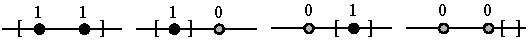
\includegraphics[width=0.55\linewidth]{./img/_vc_interval_2.pdf}
        \caption{Solutions for all the possible cases with $\vert S \vert = 2$}
    \end{figure}

    A set $S$ such that $\vert S \vert = 3$ can never be shattered.
    \begin{figure}[H]
        \centering
        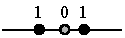
\includegraphics[width=0.13\linewidth]{./img/_vc_interval_3.pdf}
        \caption{Instance with $\vert S \vert = 3$ in which an interval cannot be found}
    \end{figure}
\end{example}

\begin{example}[Rectangles]
    Let $X = \mathbb{R}^2$ and $\mathcal{C} = \{ c: X \rightarrow \{0, 1\} \}$.
    Learning a concept $c \in \mathcal{C}$ consists of learning an axis-aligned rectangle that includes the points labeled with $1$ and excludes the ones labeled with $0$.

    It holds that $\texttt{VCD}(\mathcal{C}) = 4$ as it is possible to capture all the possible dichotomies for at least an $S$ such that $\vert S \vert = 4$.
    \begin{figure}[H]
        \centering
        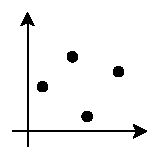
\includegraphics[width=0.15\linewidth]{./img/_vc_rectangle_4.pdf}
        \caption{
            \parbox[t]{0.7\linewidth}{
                Case with $\vert S \vert = 4$ in which any subset of the points can be enclosed within a rectangle that includes only those points
            }
        }
    \end{figure}

    For $\vert S \vert = 5$, there is at least an instance for any $S$ in which a rectangle is not possible.
\end{example}


\begin{theorem}[Sample complexity upper bound] \marginnote{Sample complexity upper bound}
    Let $\mathcal{C}$ be a concept class with $\texttt{VCD}(\mathcal{C}) = d$ where $1 \leq d < +\infty$ and
    $\mathcal{L}$ a consistent learner for $\mathcal{C}$.
    Then, for every $0 < \varepsilon < \frac{1}{2}$ and $\delta \leq \frac{1}{2}$,
    $\mathcal{L}$ is a PAC learning algorithm for $\mathcal{C}$ if it is provided with an amount $m$ of samples such that:
    \[ m \geq k_0 \left( \frac{1}{\varepsilon} \log\left(\frac{1}{\delta}\right) + \frac{d}{\varepsilon}\log\left(\frac{1}{\varepsilon}\right) \right) \]
    for some constant $k_0$.
\end{theorem}

\begin{theorem}[Sample complexity lower bound] \marginnote{Sample complexity lower bound}
    Let $\mathcal{C}$ be a concept class with $\texttt{VCD}(\mathcal{C}) \geq d$ where $d \geq 25$\footnote{
        This comes from the original proof that was done on neural networks. With a slightly modified argument, the theorem holds for $d \geq 2$.
    }.
    Then, every PAC learning algorithm for $\mathcal{C}$ requires an amount $m$ of samples such that:
    \[ m \geq \max \left\{ \frac{d-1}{32\varepsilon}, \frac{1}{4\varepsilon}, \log\left(\frac{1}{4\delta}\right) \right\} \]

    \begin{remark}
        Note that this value depends on the VC dimension $d$ which, in theory, 
        implies that it should be very difficult to learn neural networks with large \texttt{VCD} as it would require lots of data.
        
        In practice, it usually happens that the dataset has particular distributions or properties.
    \end{remark}
\end{theorem}


% \lohead{}
% \lehead{}